% ==============================================================================
% Chapter 5: Data Model & External Integration Boundaries
% Indicative Space Budget: ~2.5 pages
% Status: Draft — Prepared by Research; Pending Partner Review
% ==============================================================================

\fgchapter{05}{Chapter 05 --- Data \& Protocols}{Data Model \& External Integration Boundaries}{Transactional invariants, six-interface protocol boundaries, and analytical telemetry sizing}{sec:data-protocols}

\subsection{Conceptual Transactional Data Model and Consistency Invariants}
\label{sec:data-model}

To guarantee financial integrity across unreliable mobile networks and heterogeneous station hardware, Fuel\&Go's conceptual relational schema (PostgreSQL + PostGIS~\cite{postgis2025docs}) centers on six core entities: \texttt{DriverAccount}, \texttt{VehicleProfile}, \texttt{StationConnector}, \texttt{EnergySession}, \texttt{TelemetrySnapshot}, and \texttt{Payment\-Ledger\-Entry}. Four strict transactional invariants govern runtime consistency (\texttt{FR-05}, \texttt{FR-06a}):

\begin{itemize}[leftmargin=1.4em, itemsep=2pt]
  \item \textbf{Command Idempotency \& Downstream Limits}: Retries of the same logical operation reuse the same \texttt{idempotency\_key} (new operations receive new keys), enforced via durable deduplication (DB unique key + request hash + stored outcome) to prevent duplicate internal commands or double settlement. However, a local DB unique constraint alone does not guarantee exactly-once physical pump/charger activation if a remote start times out after reaching an operator lacking native downstream idempotency; such ambiguous timeouts must enter \texttt{RECONCILING}.
  \item \textbf{Single-Active-Session Lock}: A partial unique index on \texttt{(station\_id, bay\_id)} holds the bay reservation lock across \texttt{PREAUTH\_PENDING}, \texttt{AUTH\_\-DISPATCHED}, \texttt{FUELING\_ACTIVE}, \texttt{EV\_CHARGING\_ACTIVE}, and \texttt{RECONCILING}, preventing concurrent driver authorization on the same bay. Lock release from \texttt{RECONCILING} occurs only upon authoritative operator evidence (confirmed CDR, forecourt receipt, or verified idle/non-activated hardware status).
  \item \textbf{Append-Only Financial Ledger}: \texttt{PaymentLedgerEntry} records immutable state transitions (\texttt{PREAUTH\_HELD}, \texttt{CAPTURE\_\-SUBMITTED}, \texttt{CAPTURED}, \texttt{VOID\_\-REQUESTED}) rather than in-place updates, enabling auditable reconciliation against operator CDRs or forecourt receipts.
  \item \textbf{Zero Raw Card Data}: Only opaque PSP surrogate tokens and masked last-four display metadata are persisted (\texttt{NFR-05})~\cite{pcissc2024pcidss401}.
\end{itemize}

\subsection{Six External Integration Interfaces and Protocol Non-Interchangeability}
\label{sec:six-interfaces}

A common architectural misconception in dual-energy platforms is treating EV and forecourt protocols as interchangeable or universally deployed. In practice, Fuel\&Go's integration landscape spans \textbf{six distinct interfaces/domains}, of which four are \emph{Proposed Fuel\&Go Core Interfaces} (Boundaries~1, 2, 5, and~6) and two are \emph{External Context Only} (Boundaries~3 and~4, outside Fuel\&Go's implementation boundary):

\begin{itemize}[leftmargin=1.4em, itemsep=2pt]
  \item \textbf{OCPI vs.\ OCPP vs.\ ISO~15118 (Distinct EV Layers)}: \textbf{OCPI} (v2.2.1 / v2.3.0)~\cite{evroaming2025ocpi} connects Fuel\&Go's backend (acting as an eMSP) to charging operators or roaming hubs (Boundary~2) for Locations, Tariffs, Sessions, Commands, and CDRs. By contrast, \textbf{OCPP} (v2.0.1 / v2.1)~\cite{oca2020ocpp201,oca2025ocpp21} governs the operator's internal link between physical chargers and its Charge Point Management System (Boundary~3), while \textbf{ISO~15118-2/20}~\cite{iso15118_2_2014,iso15118_20_2022} governs vehicle-to-charger digital communication (Boundary~4; paywalled normative text not cited). Fuel\&Go does not speak OCPP or ISO~15118 directly to hardware; vehicle SoC or Plug~\&~Charge status surfaces only indirectly if the CPO exposes it upstream.
  \item \textbf{IFSF and Forecourt Heterogeneity (Boundary~5)}: Liquid-fuel forecourts rely on Forecourt Controllers (FCCs) and Point-of-Sale (POS) gateways, where \textbf{IFSF}~\cite{ifsf_specs} (member-restricted normative PDFs; architectural scope verified from public documentation) defines a common dispenser state model alongside proprietary vendor APIs. Support varies widely across legacy stations, necessitating operator-specific adapter plugins.
  \item \textbf{PSP Tokenization Boundary (Boundary~6)}: Tokenized PSP APIs under \textbf{PCI DSS v4.0.1}~\cite{pcissc2024pcidss401} isolate cardholder data from Fuel\&Go servers, narrowing compliance scope without alone establishing full PCI DSS compliance.
\end{itemize}

Table~\ref{tab:data-interfaces} consolidates the core entities, invariants, and all six interface boundaries, while Figure~\ref{fig:sequence-auth} illustrates the end-to-end authorization and settlement sequence across them.

\begin{table}[htbp]
  \centering
  \caption{Consolidated Core Data Entities, Invariants, and Six-Interface Candidate Protocol Matrix.}
  \label{tab:data-interfaces}
  \small
  \begin{tabularx}{\linewidth}{@{}P{12mm} P{32mm} P{25mm} P{25mm} L@{}}
    \toprule
    \rowcolor{fgOlive}
    \fgtableheader{ID} & \fgtableheader{Interface / Domain} & \fgtableheader{Boundary Role} & \fgtableheader{Candidate Protocol} & \fgtableheader{Primary Data Entities \& Consistency Invariants} \\
    \midrule
    \textbf{1} & Mobile app $\leftrightarrow$ Fuel\&Go backend & Proposed Fuel\&Go Core Interface & REST~\cite{rfc9110} + WebSocket~\cite{rfc6455} & \texttt{DriverAccount}, \texttt{VehicleProfile}, \texttt{TelemetrySnapshot}; client \texttt{idempotency\_key} on all mutations. \\
    \textbf{2} & Fuel\&Go backend $\leftrightarrow$ EV operator / roaming & Proposed Fuel\&Go Core Interface & OCPI v2.2.1 / v2.3.0~\cite{evroaming2025ocpi} & \texttt{StationConnector}, \texttt{EnergySession}; remote start/stop commands and CDR settlement reconciliation. \\
    \textbf{3} & Charging station $\leftrightarrow$ EV CPMS / CSMS & External Context Only & OCPP 2.0.1 / 2.1~\cite{oca2020ocpp201,oca2025ocpp21} & Outside Fuel\&Go boundary; governs charger meter values and operator-side authorization. \\
    \textbf{4} & Vehicle $\leftrightarrow$ charging station (EVSE) & External Context Only & ISO~15118-2 / 20~\cite{iso15118_2_2014,iso15118_20_2022} & Outside Fuel\&Go boundary; vehicle SoC/Plug~\&~Charge surfaced only indirectly via CPO telemetry. \\
    \textbf{5} & Fuel\&Go backend $\leftrightarrow$ forecourt / POS gateway & Proposed Fuel\&Go Core Interface & IFSF~\cite{ifsf_specs} / Vendor POS API & \texttt{EnergySession}; single-active-session bay lock; local FCC retains autonomous hardware safety cutoffs. \\
    \textbf{6} & Fuel\&Go backend $\leftrightarrow$ Payment Service Provider & Proposed Fuel\&Go Core Interface & Tokenized PSP API (PCI DSS v4.0.1~\cite{pcissc2024pcidss401}) & \texttt{PaymentLedgerEntry} (append-only); zero raw PANs; automated hold-release/void request on completion/abort. \\
    \bottomrule
  \end{tabularx}
\end{table}

% ------------------------------------------------------------------------------
% FIGURE 5.1 HOOK FOR DESIGN AGENT (TikZ Vector Diagram #4)
% Six-Interface Sequence Diagram: Mobile App, Fuel&Go Backend, PSP,
% EV Operator/CPMS (OCPI) + External Context (OCPP/ISO 15118), Forecourt Gateway (IFSF).
% ------------------------------------------------------------------------------
\begin{figure}[!htbp]
  \centering
  % ==============================================================================
% figures/sequence_auth_settlement.tex
% TikZ Vector Diagram #4 (Figure 5.1): End-to-End Authorization, Telemetry,
% and Settlement Sequence Across Six Interface Boundaries (Conceptual Design)
% Strictly <= 16.5cm wide; all labels >= 9.5pt; ZERO nested tikzpictures
% ==============================================================================
\begin{tikzpicture}[
  x=1cm, y=1cm,
  >=Stealth,
  actor/.style={
    rectangle, rounded corners=3pt,
    draw=#1, line width=1.05pt, fill=#1!12,
    minimum width=2.85cm, minimum height=0.86cm,
    align=center, inner sep=2.5pt,
    font=\fontsize{9.5pt}{10.5pt}\selectfont\bfseries, text=fgEspresso
  },
  extactor/.style={
    rectangle, rounded corners=3pt,
    draw=#1, dashed, line width=1.05pt, fill=#1!8,
    minimum width=2.95cm, minimum height=0.86cm,
    align=center, inner sep=2.5pt,
    font=\fontsize{9.5pt}{10.5pt}\selectfont\bfseries, text=fgEspresso
  },
  coremsg/.style={draw=fgTeal, line width=1.0pt, ->},
  extmsg/.style={draw=fgEspresso!85, dashed, line width=1.0pt, ->},
  msglbl/.style={font=\fontsize{9.5pt}{10.2pt}\selectfont, text=fgEspresso, fill=fgWhite, inner sep=1.2pt}
]

% ------------------------------------------------------------------------------
% 5 Lifelines (x = 1.45, 4.80, 8.15, 11.50, 14.85 -> total width <= 16.35cm)
% ------------------------------------------------------------------------------
\node[actor=fgTeal]        (m)   at (1.45, 9.25) {Mobile App\\(Client)};
\node[actor=fgTeal]        (b)   at (4.80, 9.25) {Fuel\&Go\\Backend};
\node[extactor=fgOlive]    (p)   at (8.15, 9.25) {PSP\\(Tokenized)};
\node[extactor=fgEcoGreen] (ev)  at (11.50, 9.25) {EV Operator\\CPMS (OCPI)};
\node[extactor=fgTerracotta](fc) at (14.85, 9.25) {Forecourt /\\POS Gateway};

\foreach \x in {1.45, 4.80, 8.15, 11.50, 14.85} {
  \draw[fgRuleGray, line width=0.9pt, dashed] (\x, 8.80) -- (\x, 0.45);
}

% ------------------------------------------------------------------------------
% Sequence Messages (Proposed Core Interfaces 1, 2, 5, 6 = Solid)
% ------------------------------------------------------------------------------
% 1. Mobile -> Backend (Boundary 1)
\draw[coremsg] (1.45, 8.20) -- (4.80, 8.20)
  node[msglbl, midway, above] {\textbf{[B1]} Scan Bay + Start (\texttt{idem\_key})};

% 2. Backend -> PSP (Boundary 6)
\draw[coremsg, draw=fgOlive] (4.80, 7.42) -- (8.15, 7.42)
  node[msglbl, midway, above] {\textbf{[B6]} Pre-Auth Hold Request};

% 3. PSP -> Backend (Boundary 6)
\draw[coremsg, draw=fgOlive] (8.15, 6.72) -- (4.80, 6.72)
  node[msglbl, midway, above] {\textbf{[B6]} Hold Approved (\texttt{PREAUTH\_HELD})};

% 4. EV Path: Backend -> EV CPMS (Boundary 2)
\draw[coremsg, draw=fgEcoGreen] (4.80, 5.90) -- (11.50, 5.90)
  node[msglbl, pos=0.62, above] {\textbf{[B2: OCPI]} Remote Start Command (EV Path)};

% External Context Box (Boundaries 3 & 4: OCPP & ISO 15118)
\draw[fgEcoGreen, dashed, line width=1.05pt, rounded corners=3pt, fill=fgEcoTint!75]
  (9.65, 4.58) rectangle (13.35, 5.50);
\node[anchor=center, align=center, font=\fontsize{9.5pt}{10.5pt}\selectfont, text=fgEspresso]
  at (11.50, 5.04) {\textbf{External Context Only}\\\textbf{[B3]} OCPP $\cdot$ \textbf{[B4]} ISO 15118};

% 5. Fuel Path: Backend -> Forecourt (Boundary 5)
\draw[coremsg, draw=fgTerracotta] (4.80, 4.00) -- (14.85, 4.00)
  node[msglbl, pos=0.72, above] {\textbf{[B5: IFSF / POS]} Authorize Dispenser (Fuel Path)};

% 6. Live Telemetry (Boundary 1 WebSocket)
\draw[coremsg] (4.80, 3.18) -- (1.45, 3.18)
  node[msglbl, midway, above] {\textbf{[B1: WS]} Live Telemetry (L/kWh/Cost)};

% 7. Completion & Metered Total (Boundaries 2 & 5)
\draw[coremsg, draw=fgEcoGreen] (11.50, 2.38) -- (4.80, 2.38)
  node[msglbl, pos=0.38, above] {\textbf{[B2 / B5]} Session Stop + Metered Total / CDR};
\draw[coremsg, draw=fgTerracotta] (14.85, 2.38) -- (11.65, 2.38);

% 8. Exact Capture + Automated Hold-Release Request (Boundary 6)
\draw[coremsg, draw=fgOlive] (4.80, 1.56) -- (8.15, 1.56)
  node[msglbl, midway, above] {\textbf{[B6]} Exact Capture + Hold-Release Req.\ (or \texttt{RECONCILING} on timeout)};

% 9. Digital Receipt (Boundary 1)
\draw[coremsg] (4.80, 0.82) -- (1.45, 0.82)
  node[msglbl, midway, above] {\textbf{[B1]} Digital Receipt + Final Status};

% ------------------------------------------------------------------------------
% Bottom Legend Bar
% ------------------------------------------------------------------------------
\draw[fgRuleGray, line width=0.7pt, rounded corners=3pt, fill=fgSoftCream]
  (0.0, -0.35) rectangle (16.35, 0.30);

\draw[coremsg] (0.25, -0.02) -- (1.15, -0.02);
\node[anchor=west, font=\fontsize{9.5pt}{10.5pt}\selectfont\bfseries, text=fgTeal]
  at (1.22, -0.02) {Proposed Core Interfaces: B1, B2, B5, B6 (Solid)};

\draw[extmsg, draw=fgEcoGreen] (9.15, -0.02) -- (10.05, -0.02);
\node[anchor=west, font=\fontsize{9.5pt}{10.5pt}\selectfont\bfseries, text=fgEspresso]
  at (10.12, -0.02) {External Context Only: B3, B4 (Dashed)};

\end{tikzpicture}

  \caption{End-to-End Session Authorization, Telemetry, and Settlement Sequence Across Six Interface Boundaries (\emph{Conceptual System Design}).}
  \label{fig:sequence-auth}
\end{figure}

\subsection{Analytical Telemetry Bandwidth and Latency Sizing Model}
\label{sec:sizing-model}

Because no field telemetry exists at the preliminary design stage, preliminary capacity planning relies on an explicit analytical model tagged \texttt{[Calculation]} + \texttt{[Assumption]} (all NFR targets remain provisional). Aggregate server-to-client telemetry bandwidth $B_{\text{total}}(N)$ across $N$ concurrent active sessions is modeled as:
\begin{equation}
  B_{\text{total}}(N) = N \cdot \frac{P_{\text{bytes}} \times 8}{T_{\text{interval}} \times 10^6}\;\text{[Mbps]}
  \label{eq:bandwidth}
\end{equation}
Assuming JSON WebSocket application payloads of $P_{\text{fuel}} = 512$ bytes every $T_{\text{fuel}} = 2$ s for liquid-fuel sessions ($2.048$ kbps/session) and $P_{\text{ev}} = 768$ bytes every $T_{\text{ev}} = 15$ s for EV charging ($0.410$ kbps/session), $N = 5{,}000$ concurrent sessions require $10.24$ Mbps (fueling) or $2.05$ Mbps (EV) of raw application-layer payload bandwidth. This first-order model explicitly excludes WebSocket framing, TLS record overhead, TCP/IP headers, keep-alive heartbeats, reconnect bursts, and control-plane traffic, which must be provisioned separately during infrastructure sizing.

Conversely, end-to-end authorization latency $L_{\text{auth}} = L_{\text{client-gw}} + \allowbreak L_{\text{orchestrator}} + \allowbreak L_{\text{psp-hold}} + \allowbreak L_{\text{operator-cmd}}$ is dominated by external round-trips. Under illustrative assumptions ($150\;\text{ms}$ edge, $120\;\text{ms}$ orchestrator, $900\;\text{ms}$ PSP pre-auth, and $1{,}200\;\text{ms}$ forecourt or $1{,}800\;\text{ms}$ EV roaming command), total authorization spans $2.37\;\text{s}$ (fuel) to $2.97\;\text{s}$ (EV)---exceeding NN/g's $1.0\;\text{s}$ unbroken-flow threshold~\cite{nielsen1993responsetimes} and mandating explicit mobile progress indicators.

% ------------------------------------------------------------------------------
% FIGURE 5.2 HOOK FOR DESIGN AGENT (Reproducible Python Plot #2)
% Script: scripts/plots/fig5_2_telemetry_sizing.py
% Panel A: Bandwidth scaling (Mbps) vs Concurrent Sessions N in [100..5000]
%          for Fueling (512B/2s) vs EV (768B/15s).
% Panel B: Illustrative Authorization Latency Budget decomposition (ms) vs
%          NN/g 1.0s UX guidance line.
% Required Provenance Tag: [Calculation] + [Assumption] (Not Empirical Field Data)
% ------------------------------------------------------------------------------
\begin{figure}[!htbp]
  \centering
  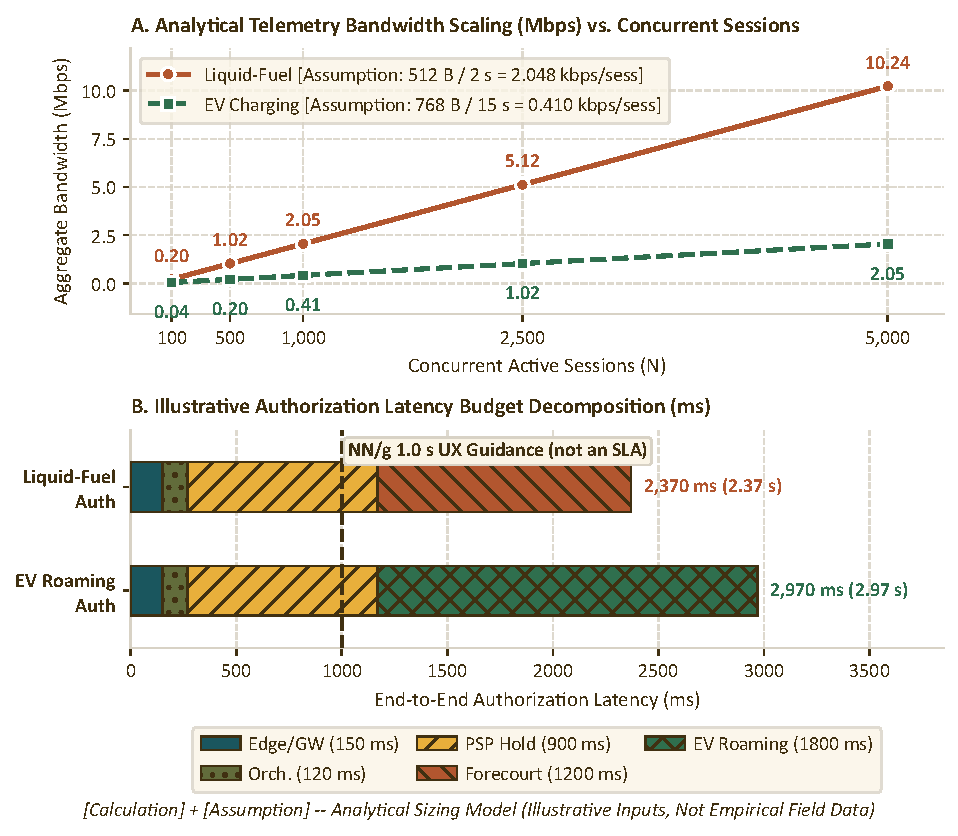
\includegraphics[width=0.88\linewidth]{figures/fig5_2_telemetry_sizing.pdf}
  \caption{Analytical Telemetry Bandwidth Scaling and Illustrative Authorization Latency Budget. \emph{Provenance}: \texttt{[Calculation]} derived from stated engineering \texttt{[Assumption]} inputs (not empirical field measurements); NN/g $1.0\;\text{s}$ UX guidance~\cite{nielsen1993responsetimes} shown for reference.}
  \label{fig:telemetry-sizing}
\end{figure}
